% Intended LaTeX compiler: xelatex
\documentclass[a4paper, 12pt]{article}
\usepackage{graphicx}
\usepackage{longtable}
\usepackage{wrapfig}
\usepackage{rotating}
\usepackage[normalem]{ulem}
\usepackage{amsmath}
\usepackage{amssymb}
\usepackage{capt-of}
\usepackage{hyperref}
\usepackage[danish]{babel}
\usepackage{mathtools}
\usepackage[margin=2.0cm]{geometry}
\hypersetup{colorlinks, linkcolor=black, urlcolor=blue}
\setlength{\parindent}{0em}
\parskip 1.5ex
\author{Jacob Debel}
\date{Fysik C \& B}
\title{Lys og bølger\\\medskip
\large Konstruktion - Brydning}
\hypersetup{
 pdfauthor={Jacob Debel},
 pdftitle={Lys og bølger},
 pdfkeywords={},
 pdfsubject={},
 pdfcreator={Emacs 29.4 (Org mode 9.6.15)}, 
 pdflang={Danish}}
\begin{document}

\maketitle
På nedenstående tegning\footnote{Kilde: Benoni og Elverkjær, FysikABbogen.} ses, hvordan lys brydes i overgangen mellem to materialer.

\begin{center}
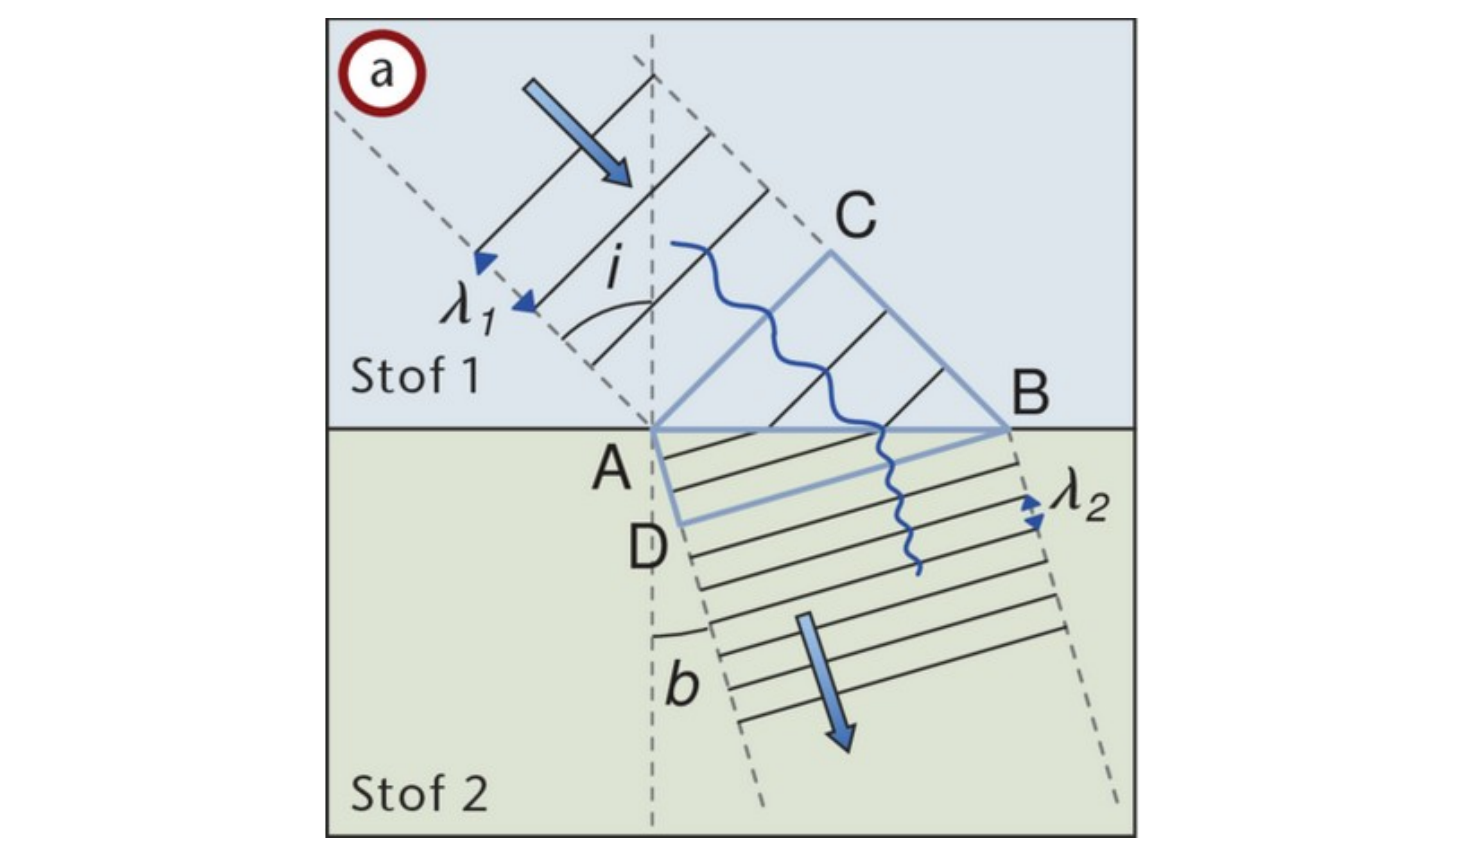
\includegraphics[width=.9\linewidth]{./img/brydning.png}
\end{center}

\begin{itemize}
\item Tegn de markerede trekanter (blå) tydeligere op.

\item Angiv henholdsvis de rette vinkler og indfaldsvinklen og brydningsvinklen i de to fremkomne trekanter.

\item Tæl hvor mange hele bølgelængder lyset udbreder sig med i hver af trekanterne.
\end{itemize}

På baggrund af ovenstående tegning og jeres skitser, \textbf{skal I nu udlede brydningsloven}.


\begin{itemize}
\item I skal bruge så korte og præcise formuleringer, som I magter. Husk at bruge de korrekte fagudtryk.
\item \textbf{I må gerne bruge jeres noter, men ikke bogen.}
\item \textbf{Tegninger, skitser og udledninger skal afleveres.}
\end{itemize}
\end{document}
